\documentclass[12pt,a4paper]{scrartcl}
\usepackage[utf8]{inputenc}
\usepackage{amsmath, amssymb, amsfonts}
\usepackage{graphicx}
\usepackage[top=3cm, bottom=2.5cm, left=3cm, right=4cm]{geometry}\usepackage[english,german]{babel} 
\usepackage{csquotes}
\usepackage{hyperref}

\usepackage[style=ieee]{biblatex}
 
\graphicspath{ {./media/} } 
\parindent 0px
\linespread{1.25} %gleich wie 1.5 in word
\pagestyle{headings}


\addbibresource{ref.bib}

\begin{document} \selectlanguage{german}
\begin{titlepage}
 
  \null\vfill
  \begin{center}
    GYMNASIUM OTTOBRUNN
    \vskip 2em
    Oberstufenjahrgang 2023/2024
    \vskip 2em
    Seminar: \\ Die Welt der Mathematik - die Mathematik in der Welt
    \vskip 1em
    Leitfach: Mathematik
    
    \vskip 5em
    Exposé zur Seminararbeit
    \vskip 2em
    
    {
      \usekomafont{title} \LARGE
        Der RSA - Algorithmus und seine Anwendung in der IT-Sicherheit
      \par
    }
     
    \vskip 4.5em
    
  \end{center}
  Verfasser: \hspace{1cm} Julian Thanner
  \vskip 0.5em
  Seminarleiterin: StDin Birgit Gregor
  \vskip 2em
  Bewertung: .............. Punkte
  \vskip 1em
  Unterschrift der Seminarleiterin: \underline{\hspace{5cm}}
 \end{titlepage}
	
\thispagestyle{empty}
\tableofcontents
\thispagestyle{empty}


\pagebreak
\section{Einleitung}

\subsection{Die symmetrischen Verschlüsselung}

Bei symmetrischen Verschlüsselungsverfahren gibt es, anders als bei asymmetrischen Verfahren (auch: Public Key Verfahren), nur einen Schlüssel für die Ent- und Verschlüsselung. Diese bieten viele Vorteile, wie zum Beispiel eine kurze Schlüssellänge oder auch eine deutlich kleinere Verschlüsselungszeit. Allerdings kommt die symmetrische Verschlüsselung auch mit einigen Nachteilen, unteranderem "setzt [sie] voraus, dass Sender und Empfänger einer Nachricht, und nur diese beiden ein gemeinsames
Geheimnis den sogenannten Schlüssel, besitzen." \cite[S. 7]{schwenk2010sicherheit}. Das stellt aber in der Praxis als ein Problem dar, weil es nicht immer möglich ist sich vor der ersten verschlüsselten Kommunikation persönlich zu treffen, dies aber für eine symmetrische Verschlüsselung nötig ist. Dafür wird eine andere Verschlüsselungsmethode benötigt, ein sogenanntes Public Key Verfahren. Hier liegt der Vorteil darin, das es einen öffentlichen und einen privaten Schlüssel gibt. Die Nachricht kann dann mit dem öffentlichen Schlüssel einer Person verschlüsselt und dann nur mit dem privaten Schlüssel wieder entschlüsselt werden. Ein Algorithmus dafür ist der RSA-Algorithmus, den ich im folgenden erklären möchte.

\pagebreak


\section{Begriffserklärungen}
	\subsection{Modulo Operation} %Notwendigkeit?
	Die Modulo Operation gibt den Rest einer ganzzahligen Division zurück.
	$$ {7 \bmod 4 = 3} $$
	$$ {16 \bmod 3 = 1} $$
	
	\subsection{Multiplikatives Inverses}
	"Das multiplikativ inverse Element $a^{-1}$ eines Elements a in der Gruppe $\mathbb{Z}_n ^*$ ist das eindeutig bestimmte Element, für das gilt $${a^{-1} * a  =  a * a^{-1}  =  1}$$ wobei 1 das neutrale Element der Gruppe ist." \cite{hwlang} \\
	
	So ist zum Beispiel das multiplikative Inverse $a$ von 3, $a=2$, weil: \\
	${3 * 2 = 6 = 1 \bmod 5}$ \\
	
	Für das Beispiel ${5 * a = 1 \bmod 5}$ wäre $a=5$, weil \\
	${5 * 5 = 25 = 1 \bmod 5}$ \\
	
	\subsection{Einwegverschlüsselungsverfahren}
	Mithilfe eines Einwegverschlüsselungsverfahrens (auch Hashfunktion) kann anhand eines beliebig großem Quelltext eine Prüfsumme erzeugt werden, welche in der Regel eine fest definierte Länge hat. Man könnte eine Hashfunktion auch mit einem Fingerabdruck vergleichen. Ein gutes Beispiel für eine Einwegfunktion, wäre die Modulo-Operation, da sich hier aus dem Ergebnis nicht feststellen lässt, aus welchen Zahlen das Ergebnis berechnet wurde. \\
	Zum Beispiel haben die Modulo Operation: ${14 \bmod 6}$  und diese: ${20 \bmod 3}$ beide als Ergebnis 2. Es lässt sich aber nicht zurückschließen mit welchen Zahlen die Modulo Operation durchgeführt wurde, da es dafür unendlich viele Fälle gibt. Es gibt aber noch einige weitere Einwegfunktionen, wie z.B. MD5 oder SHA-256. Diese haben unteranderem die folgenden Anwendungen:
	
	%TODO Anwendungen Ausformulieren
	\begin{itemize}
	\item
	
	\end{itemize}
	
	\label{ch:einweg}
	\subsection{Eulersche $\phi$ Funktion}
	\label{cha:phi}
	
	Die Eulersche $\phi$ Funktion gibt für jede natürliche Zahl ${n > 0}$ an, wie viele positive natürliche Zahlen es gibt, die teilerfremd zu n sind. Das heißt der größte gemeinsame Teiler dieser Zahlen ist 1. Zum Beispiel ist ${\phi(9) = 6}$, da ${9}$ nicht durch ${2, 4, 5, 6, 7 }$ und $8$ teilbar ist. Bei Primzahlen ist die $\phi$ Funktion sehr einfach zu berechnen, da diese nur durch sich selber und 1 teilbar sind. Somit gilt: $${\phi(p) = p - 1}$$
	Nochdazu ist diese Funktion Multiplikativ, also gilt: ${\phi(p * q) = \phi(p) * \phi(q)}$.
	Daraus folgt, das für Primzahlen gelten muss:
	$${\phi(p * q) = (p - 1) * (q - 1)}$$
	
	Somit ist es sehr einfach $\phi(n)$ zu berechnen, wenn $p$ und $q$ Primzahlen sind.
	\subsection{Satz von Euler}
	Nur wenn zu wenig text
	
	\subsection{Der euklidische Algorithmus}
	 Mit dem erweiterten Euklidischen Algorithmus kann der größte gemeinsame Teiler ggT(a,b) von zwei ganzen Zahlen a und b berechnet werden.
	 Dabei wird in jedem Schritt $a / b = q$ gerechnet. Dabei wird nach jedem Schritt $a=b$ und $b = r$ gesetzt. $r$ ist dabei der Rest der division. Die Iteration endet, wenn $b=0$. Der größte gemeinsame Teiler ggT(a, b) ist dann $a$. Im Folgenden wird das ganze mit einem Beispiel, wo $a = 74$ und $b = 38$ ist. \\
	 \begin{tabular}{ c c c c c c c}
 		a & : & b & = & q & & r \\ 
 		74 & : & 38 & = & 1 & Rest & 36\\ 
 		38 & : & 36 & = & 1 & Rest & 2\\ 
 		36 & : & 2 & = & 18 & Rest & 0\\
 		2 & : & 0 & \\
	\end{tabular}\\
	Bei diesem Beispiel wäre der ggT(a, b) nun 2.

	
\pagebreak
\section{Der RSA - Algorithmus}
		
	\subsection{Schlüsselgenerierung}
Die für den RSA-Algorithmus benötigten Schlüssel können sehr einfach generiert werden. Der Verschlüsselungsschlüssel besteht dabei aus $(e, n)$ und er Entschlüsselungsschlüssel besteht aus $(d, n)$. Dabei steht $e$ für encryption und $d$ für decryption 
\begin{itemize}
\item Als erstes werden zwei Primzahlen $p$ und $q$ gewählt, in einer reelen Anwendung sollte hierbei auf die in \ref{chap:primnumberselection} genannten Anforderungen geachtet werden  
\item Mit diesen wird dann $n$ aus dem Produkt von $p$ und $q$ berechnet
\item Danach wird eine große zufällige Zahl $d$ gewählt, welche teilerfremd zu ${\phi(n)}$\footnote{Zur einfachen Berechnung von ${\phi(n)}$ siehe \ref{cha:phi}} ist, das heißt:
$${ggT(d, \phi(n)) = 1}$$ 
\item Nun wird \textit{e} so berechnet, dass es das multiplikative Inverse von \textit{d} ist:
$${e * d = 1 \bmod \phi(n)}$$
\end{itemize}

\begin{figure}
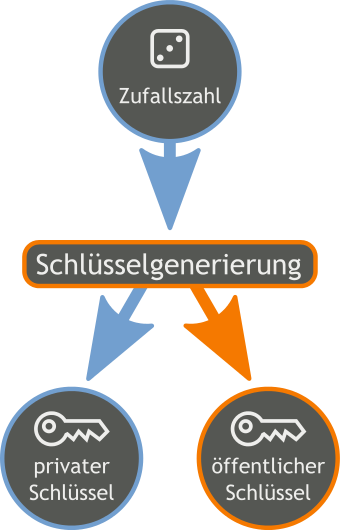
\includegraphics[scale=0.3]{Orange_blue_public_private_keygeneration} \\
\caption{Schlüsselgenerierung (aus \cite{wikipedia})}
\label{fig:figure1}
\end{figure}

Jetzt hat man den Verschlüsselungsschlüssel bestehend aus $(e, n)$ und den Entschlüsselungsschlüssel $(d, n)$. \\
$p$, $q$ und $\phi(n)$ sollten geheim gehalten bzw vernichtet werden, da diese Rückschlüsse auf $d$ möglich machen.
	
	\subsection{Ver- und Entschlüsselung}
	Als erstes müssen wir unsere Nachricht auf eine Länge zwischen 0 und $n-1$ bringen. (Für längere Nachrichten siehe \ref{cha:hole_text})
	Zum Verschlüsseln unserer Nachricht \textit{m} werden nun der öffentliche Schlüssel ($e, n$) und $m \in \mathbb{N}$ benötigt. (\textit{e} und \textit{n} sind hierbei positive Zahlen)\footcite[][6]{rsaOriginalPaper} Danach wird \textit{m} wie folgt in \textit{c} verschlüsselt: 
	$$c = m^e \bmod n$$
	Für die Entschlüsselung wird der gleiche Prozess wiederholt, nur das für \textit{m} diesmal \textit{c} verwendet wird und anstatt \textit{e} wird dann \textit{d} verwendet:
	$$m = c^d \bmod n$$
	
	\begin{figure}
	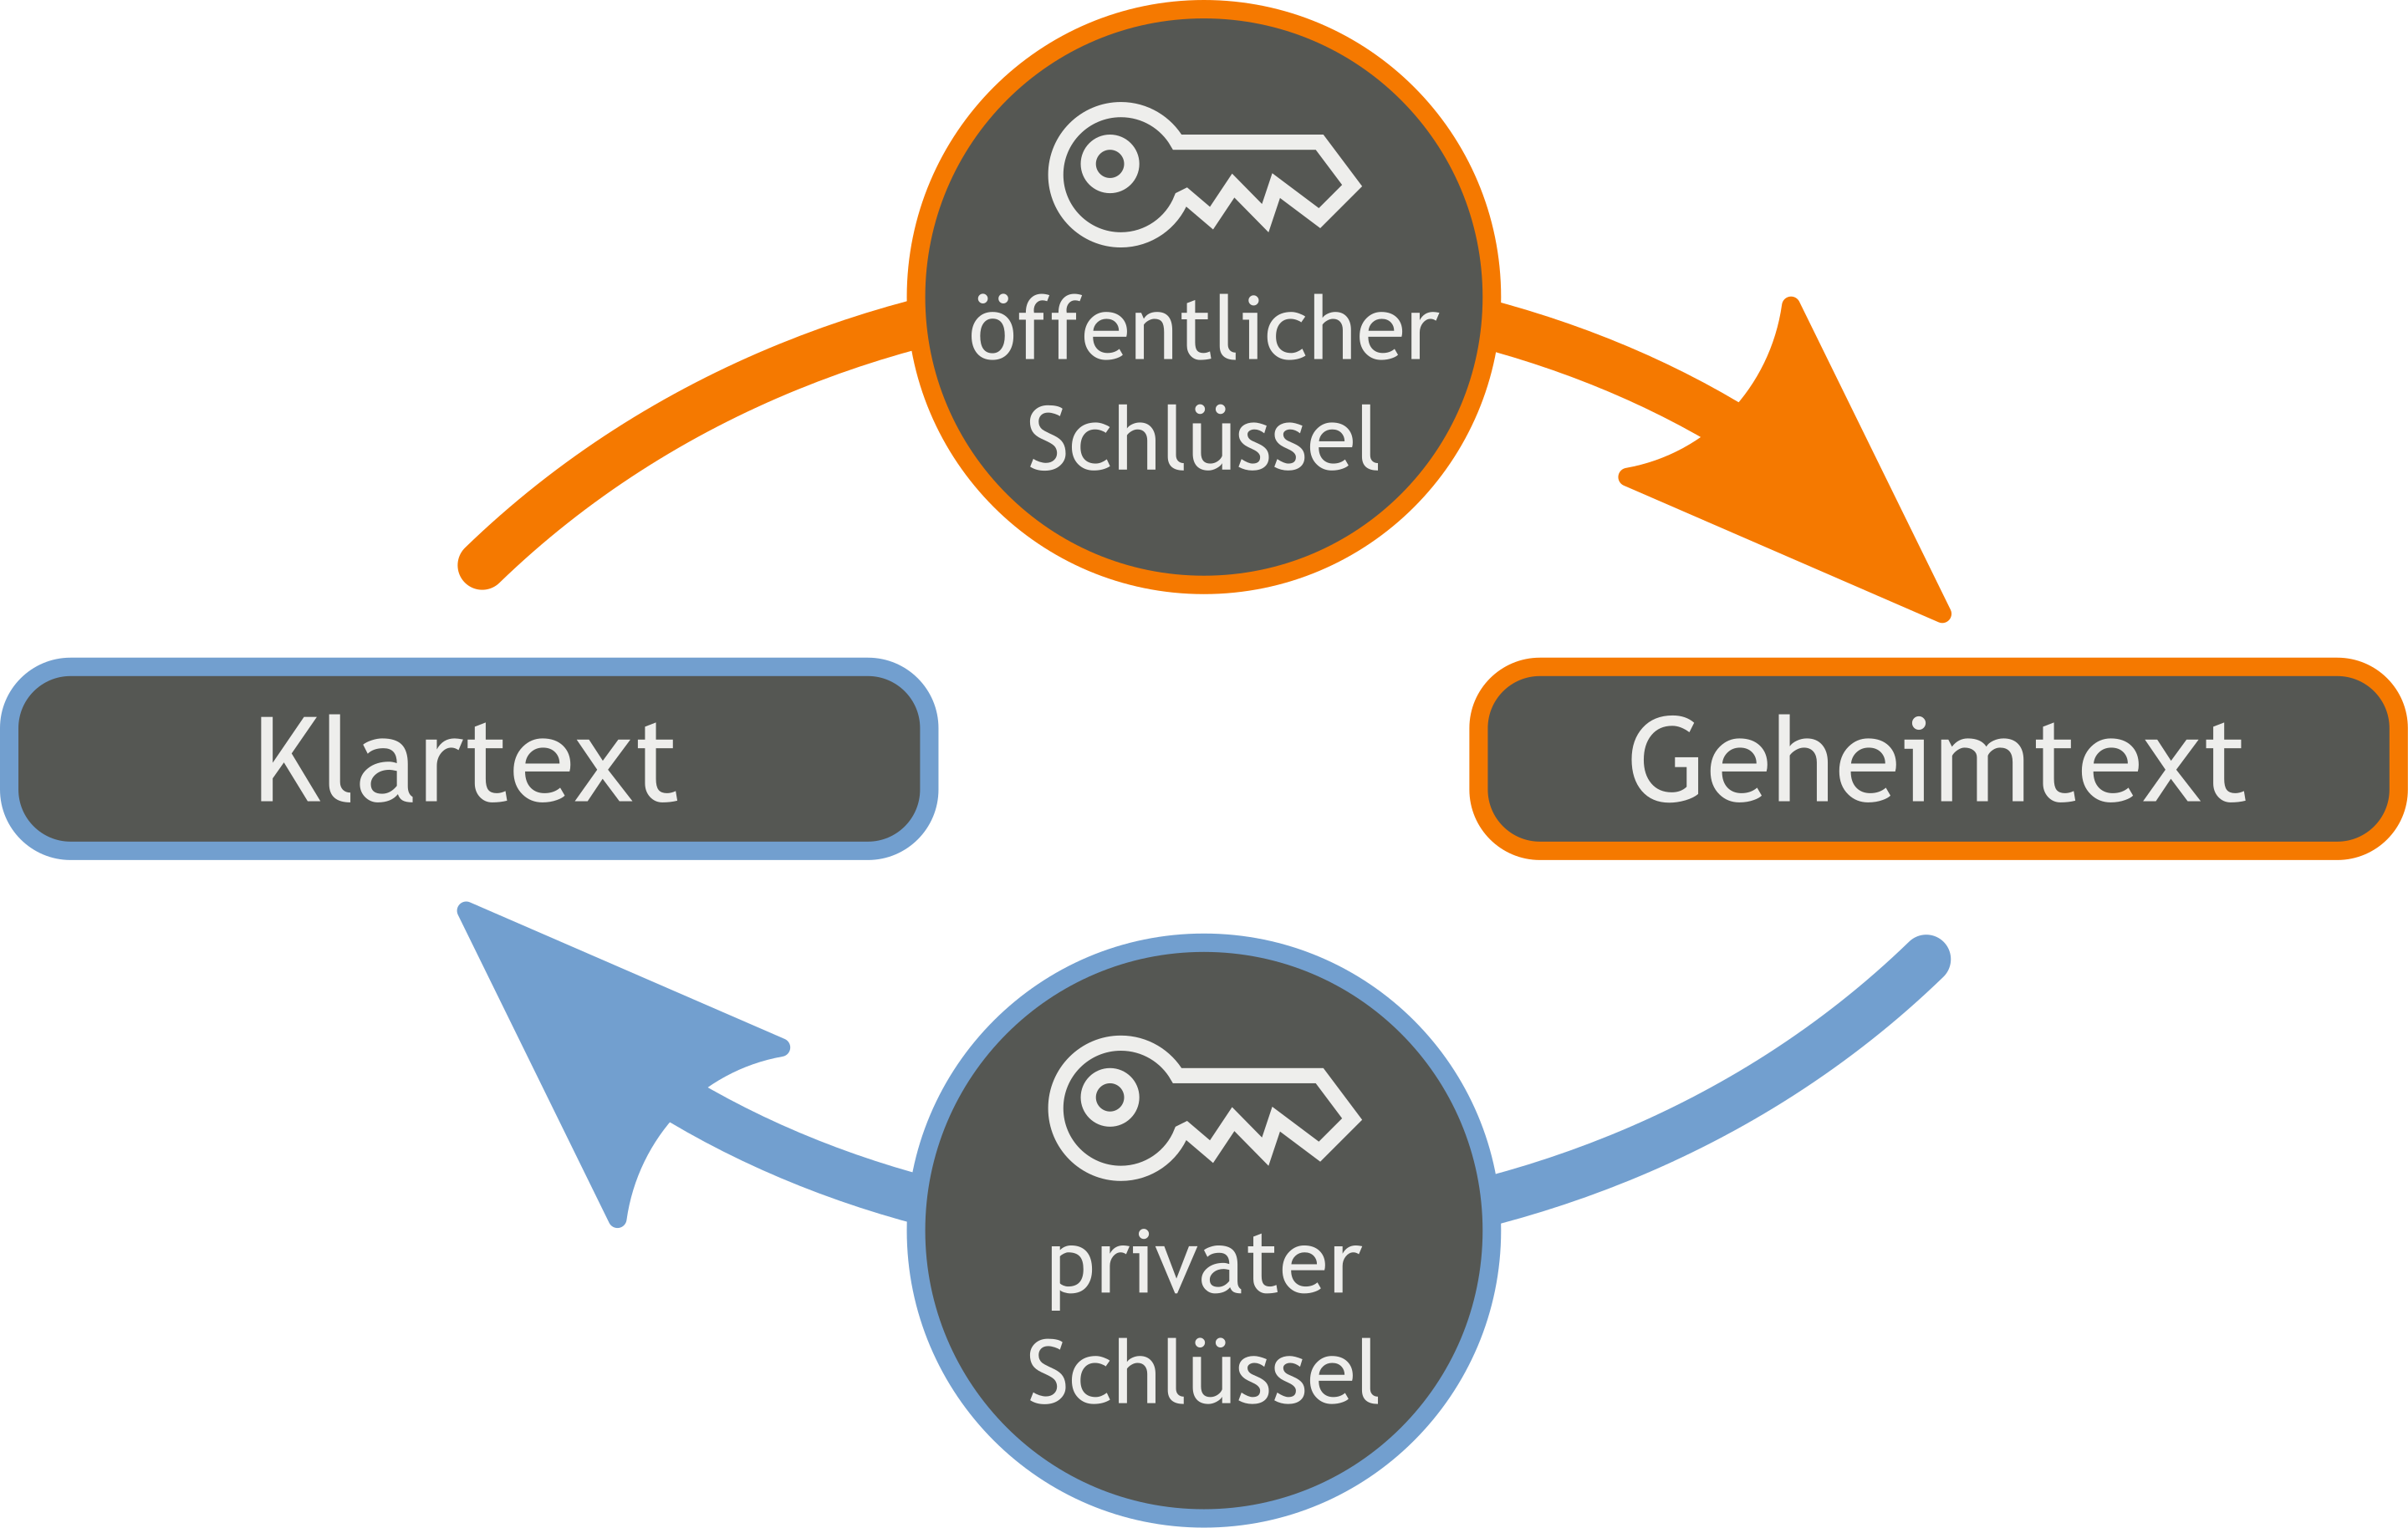
\includegraphics[scale=0.05]{Orange_blue_public_key_cryptography_de.svg.png} \\
	\caption{Der Ver- und Entschlüsselungsprozess (aus \cite{wikipedia})}
	\label{fig:figure1}
	\end{figure}
	
	Als Beispiel verschlüsseln wir die Zahl $m = 76$. Hierbei sind $e=65537$ und $n=143$.

	\begin{equation}
	\begin{split}
	c & = m^e \bmod n \\
	 &  = 76^{65537} \bmod 143 \\
 	& = 98
	\end{split}
	\end{equation}
	Unsere Verschlüsselte Nachricht ist nun also $c = 98$. Um daraus wieder \textit{m} zu berechen brauchen wir jetzt noch $d$.

	\begin{equation}
	\begin{split}
	m & = c^d \bmod n \\
	 &  = 98^{113} \bmod 143 \\
 	& = 76
	\end{split}
	\end{equation}

	\subsection{Die Mathematik hinter dem RSA-Algorithmus}
	Um verstehen zu können, warum RSA funktioniert, muss man mathematisch die Gültigkeit der Gleichung
	\begin{equation}\label{eq:fermat}
 m = c^d \bmod n
 \end{equation}

 beweisen, sodass $c^d \bmod n$ wieder $m$ ergibt. Dafür wird der Satz von Euler-Fermat benutzt: \\
	Sind a und n teilerfremde Zahlen mit $1 < a < n$, so gilt
	$$a^{\phi (n)} \equiv 1 \bmod n $$
	
	Dieser Satz soll hier nicht bewiesen werden, sondern es soll im folgenden die Gleichung (\ref{eq:fermat}) bewiesen werden, wenn $x \neq p$ und $x \neq q$ gilt, da für den Satz von Euler-Fermat $x$ und $n = p*q$ teilerfremd sein müssen. $x$ stellt hierbei unsere Nachricht m und y unsere verschlüsselte Nachricht c da. \\
	Es folgt also:
	
	\begin{align*}
	 y^d \bmod n & = (x^e \bmod n)^d \bmod n & \\
	 & = (x^e)^d \bmod n &\\
 	 & =x^{ed} \bmod n &  \parbox[t]{4cm}{e ist das multiplikative Inverse zu d, also $e * d \bmod m \equiv 1$ es folgt also daraus, dass es kein $k \in \mathbb{Z}$ gibt, so dass $e*d=k*m+1$}\\
 	 & =x^{k*m+1} \bmod n & \\
 	 & =x^{k*m}*m \bmod n & \\
 	 & =((x^m)^k \bmod n) * (x \bmod n) \bmod n & \\
 	 & =(x^m \bmod n)^k * (x \bmod n) \bmod n & \\
 	 & =(1^k \bmod n) * (x \bmod n) \bmod n &  \parbox[t]{4cm}{wegen des Satzes von Euler-Fermat (sofern x und n teilerfremd sind), da $m = (p - 1)(q - 1) = \phi(n)$ gesetzt wurde} \\
 	 & = 1 * x \bmod n & \\
 	 & = x &
 	\end{align*}

	Mit dieser Umformung konnte die Gleichung \ref{eq:fermat} bewiesen werden 
	
	\subsection{Verschlüsselung ganzer Texte}
		\label{cha:hole_text}

	Die Schwierigkeit, ganze Texte zu verschlüsseln, liegt darin, dass die Nachricht $m$ nicht großer als $n - 1$ sein darf. Eine Möglichkeit dieses Problem zu umgehen ist es die Nachricht in verschiedene kleine Blöcke zu unterteilen und dann jeden Block einzeln zuverschlüsseln. Das hat aber immer noch den Nachteil, dass der RSA Algorithmus sehr langsam ist, und deshalb für eine große Nachricht $m$, auch wenn sie in kleine Blöcke unterteilt ist, sehr lange brauchen würde. Eine sinnvollere, und auch weit aus verbreitete Lösung ist es mit dem RSA Algorithmus einen symmetrischen Schlüssel zu verschlüsseln, mehr dazu in Kapitel \ref{cha:hybrid}.


\section{Mögliche Angriffspunkte}
	\subsection{Primfaktorzerlegung}
	Es ist sehr schwierig eine Zahl $n$, die keine Primzahl ist, in ihre Primfaktoren zu zerlegen. Aktuell gibt es keinen Algorithmus, der dies für sehr große Zahlen bewältigen kann. Sollte es einen Algorithmus geben, der die Primfaktorzerlegung in sehr kurze Zeit bewältigen kann, würde das heißen, dass der RSA-Algorithmus nicht mehr sicher ist, da man sich dann sehr leicht $p$ und $q$ aus dem immer veröffentlichten $n$ berechnen kann und somit alle Schlüssel berechnen kann.
	
	Zum Beispiel benötigt der Quadratic Sieve Algorithmus aktuell um eine Zahl mit 512 Bits zu zerlegen aktuell bei 200.000.000 Befehle pro Sekunde in etwa 11700 Jahre. \cite[S. 115]{Beutelspacher2015-jl}
	Aktuell wird ein Schlüssel mit mehr als 3000 Bits als sicher angesehen. \cite[29]{bsireco}
	%TODO erklärung bit größe
	 
	\subsection{Monoalphabetische Verschlüsselung}
	Sehr einfachen Kryptosystem, wie z.B. die Caesar-Verschlüsselung, setzen oftmals auf eine Monoalphabetische Verschlüsselung, das heißt es wird jedem Buchstaben ein anderer Buchstabe zugeordnet. Wenn man immer einzelne Buchstaben mit dem RSA-Algorithmus verschlüsselt, hat man das Problem, das diese immer dem gleichen verschlüsselten Buchstaben zugeordnet werden. (Wie in Grafik \ref{fig:figure4} bei A und B zu sehen). Dadurch ist die Verschlüsselung dann nicht mehr sicher und kann sehr einfach mit Hilfe von statistischen Tabellen über die Häufigkeit eines Buchstabens geknackt werden. \footnote{Für mehr Infos dazu siehe \cite{mono}}
	
	Um diese Schwachstelle zu beseitigen, kann man anstatt einzelne Buchstaben zu verschlüsseln, ganze Blöcke an Buchstaben verschlüsseln. Hierbei ist zu beachten, dass jeder Block, umgerechnet in eine Zahl, kleiner als \textit{n} sein muss. Jetzt ist es nicht mehr möglich Rückschlüsse auf die verwendeten Buchstaben zu machen, z.B. wurden bei den unteren beiden Beispielen in Abbildung \ref{fig:figure4} nur A und B getauscht und es kommt eine ganz andere Zahl raus.


\begin{figure}		
\includegraphics[scale=0.45]{rsa_mono} \\
\caption{Verschlüsselung verschiedener Buchstaben mithilfe des ASCII Standards und des RSA-Algorithmus}
\label{fig:figure4}
\end{figure}
	
\subsection{Die Wahl der Primzahlen}
\label{chap:primnumberselection}
Wahrscheinlich entfernen

 nicht zu nah beieinander \cite{rowland} \\

\pagebreak

\section{Anwendungsbereiche in der IT - Sicherheit}
	\subsection{Digitale Nachrichten}
Um eine Nachricht, hier genannt \textit{m}, mit einem Computer verarbeiten zu können, muss diese erst in Zahlen umgewandelt werden. Dafür existiert der ~ASCII~ Standard, mit dem Computer Buchstaben in Zahlen umwandeln können. Jede Nachricht \textit{m} muss kleiner sein als \textit{n}. In der Realität spielt das allerdings keine Rolle, da normalerweise Werte für \textit{n} mit mehr als 100 Stellen verwendet werden und der normale ASCII Standard 7-Bit Werte und der erweiterte ASCII Standard 8-Bit Werte verwendet.\footnote{7-Bit hat Zahlen bis 128, 8-Bit bis 256}
	
	\subsection{Digitale Signatur}
	Der RSA-Algorithmus kann auch genutzt werden, um Nachrichten zu signieren. Durch das Signieren von z.B. Emails kann der Empfänger sicherstellen, dass die Nachricht von dem Besitzer des zugehörigen privaten Schlüssels verschickt wurde. Diese Funktion der Signatur wird auch genutzt, um die Fälschungssicherheit und Originalität von  Dokumenten sicherzustellen. Um bei einer Signatur nicht die Länge der Nachricht zu verdoppeln, wird diese mithilfe einer Einwegfunktion auf eine vordefinierte Länge gebracht.\footnote{Siehe Kapitel \ref{ch:einweg} auf Seite \pageref{ch:einweg}}\\

Als erstes wandelt man die Nachricht mithilfe eines Standards in Zahlen um. Mithilfe eines Hashing-Algorithmus wird nun der Hash-Wert der zu signierenden Nachricht berechnet. Dieser Wert wird dann mit dem privaten Schlüssel, dem Encryption-Key, der normalerweise der öffentliche Schlüssel ist, verschlüsselt. %Schöner formulieren
	Der Decryption-Key wird dann, anders als wenn man eine geheime Nachricht versenden will, veröffentlicht.\\
	Die originale Nachricht wird dann zusammen mit der digitalen Signatur verschickt und der Empfänger entschlüsselt diese dann mithilfe des öffentlichen Schlüssels wie folgt:\\
	Als erstes generiert der Empfänger mithilfe des Hash-Algorithmus einen Hash-Wert von der Nachricht, die auf ihre Echtheit überprüft werden soll. Dann wird mit dem öffentlichen Schlüssel des Senders der, an die Nachricht angehängte, verschlüsselte Hash-Wert des Senders entschlüsselt. \\
Wenn der generierte und der entschlüsselte Hash-Wert übereinstimmen, kann sicher festgestellt werden, dass die Nachricht nicht verändert wurde. \\
Wenn z.B. jetzt eine dritte Person die Nachricht abändern würde, würde ein anderer Hash-Wert beim Empfänger für diese Nachricht herauskommen, da der Hash-Algorithmus schon bei der Änderung eines einzelnen Bits einen anderen Hash-Wert ausgibt. Wenn dieser dann mit dem verschlüsselten Hash-Wert verglichen wird, kann festgestellt werden, ob die Nachricht im Original vorliegt, denn wenn dem nicht so ist stimmen die Hash-Werte nicht mehr überein.\\


%TODO wenn noch mehr text  --> https/tls

\begin{figure}
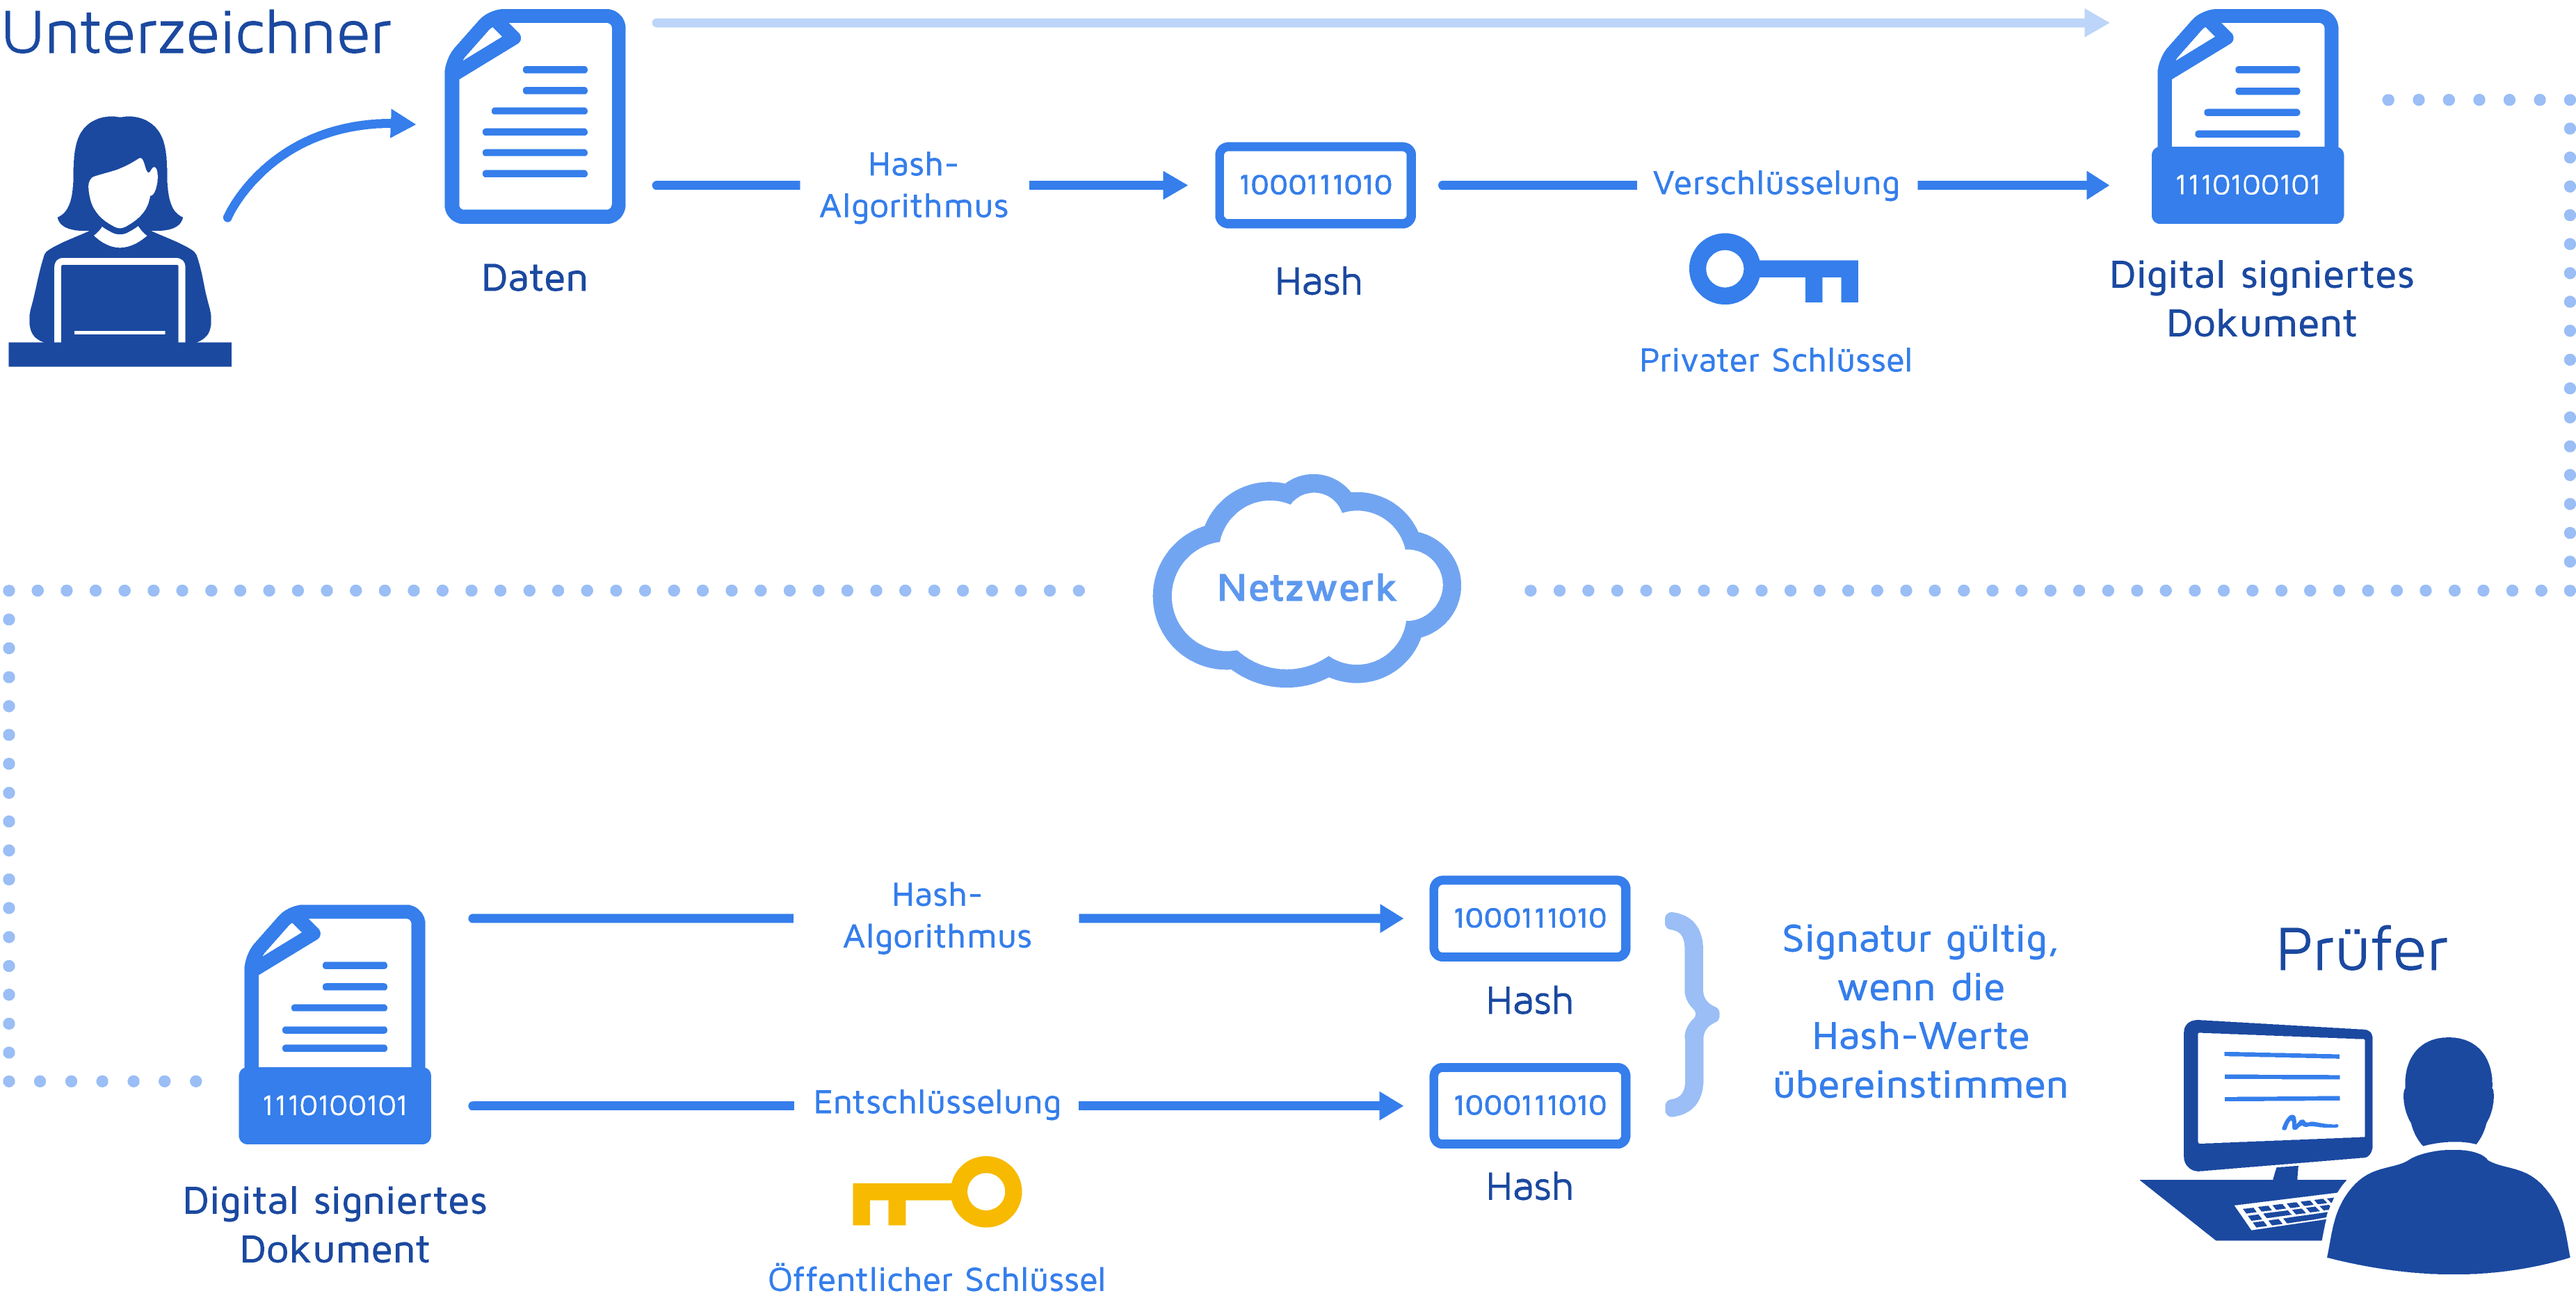
\includegraphics[scale=0.45]{Dokument_digitale_Signatur} \\
\caption{Ein Dokument digital signieren (aus \cite{digitalsignature})}
\label{fig:figure3}
\end{figure}

Das ganze funktioniert dann wie folgt:

Als erstes berechnet man den Hash-Wert mithilfe einer Einwegfunktion:
$$ {h = e(m)} $$

Dann berechnet man mit dem RSA-Algorithmus die Signatur \textit{s}
$$ {s = h^e \bmod n} $$

Diese Signatur wird dann an die Nachricht angehängt und dann wird diese veröffentlicht.
Der Empfänger kann dann mit den folgenden Schritten die Integrität der Nachricht sicherstellen:

Als erster wird erneut h von der empfangenen Nachricht $m$ bestimmt:
$${h_{empfangen} = e(m) }$$
Dann muss die Signatur wieder entschlüsselt werden:
$$ {h_{entschluesselt} = s^d \bmod n} $$
Anschließend werden diese beiden Hashwerte verglichen und wenn diese gleich sind, kann man davon ausgehen, dass die Nachricht nicht verändert wurde. \\


Beispiel: Die digitale Signatur von \textit{m} = 8:\\ 
Angenommen:
$${ \textit{m} = 8 }$$
$${ \textit{n} = 187 }$$
$${ \textit{d} = 59 }$$
$${ \textit{e} = 19 }$$


Erst wird der Hash-Wert von \textit{m} berechnet...
$$ {16 = e(8)} $$	

...und dann mit der RSA-Funktion verschlüsselt: %richtige Formulierung?
$$ {152 = 16^19 \bmod 187} $$	

Um jetzt sicherzustellen, dass die Nachricht nicht verändert wurde, wird erneut der Hash Wert berechnet:
$$ {16 = e(8)} $$	
und dann die Signatur $s$ entschlüsselt:
$$ {16 = 152^59 \bmod 187} $$

Und jetzt werden diese Beiden wieder verglichen und es wird ersichtlich, das $m$ nicht verändert wurde.


	 	
	\subsection{Hybride Verschlüsselung}
		\label{cha:hybrid}
		\begin{figure}
		
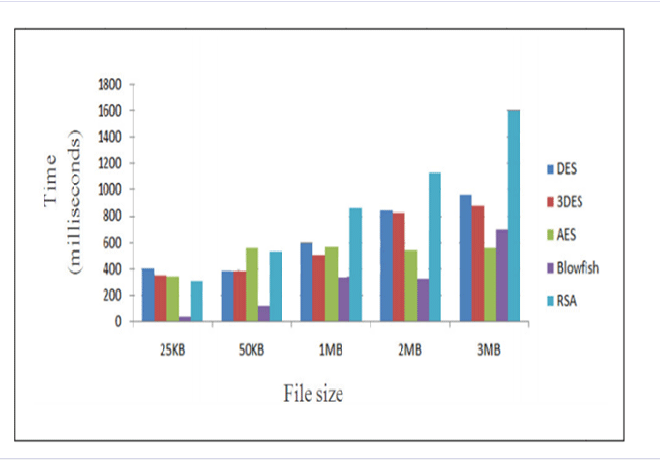
\includegraphics[scale=0.45]{rsa_time} \\
\caption{Decryption time vs. File size for DES, 3DES, AES, Blowfish and RSA (aus \cite{rsatime})}
\label{fig:figure5}
\end{figure}
		
		Wenn man große Texte bzw. Dateien verschlüsseln möchte, brauchen verschieden Algorithmen unterschiedlich lange. Bei der Verschlüsselung mit dem RSA-Algorithmus entsteht das große Problem, dass dieser für immer größer  werdende Texte immer länger braucht, wie in Abbildung \ref{fig:figure5} zu sehen ist. 

		Hierfür kann dann das Konzept der hybriden Verschlüsselung genutzt werden. Dabei kombiniert man eine asymmetrisches und eines symmetrisches Verschlüsselungsverfahren. Diese bringt den Vorteil mit sich, dass die Vorteile  beider Verfahren kombiniert werden können. Das ganze hat aber auch einige Nachteile z.B. muss man dafür beide Verfahren implementieren und die Sicherheit der hybriden Verschlüsselung ist jetzt abhängig von zwei verschiedenen Verschlüsselungsalgorithmen. \\
		Um nun eine Nachricht verschlüsselt versenden zu können, ohne lange auf die Verschlüsselung warten zu müssen, wird als erstes ein symmetrischer Schlüssel zufällig generiert werden. Mit diesem wird dann die Nachricht verschlüsselt. Dann wird der asymmetrisch verschlüsselte symmetrische Schlüssel zusammen mit der verschlüsselten Nachricht versendet.


\pagebreak
\section{Anhang}

\listoffigures
\pagebreak

\nocite{*}
\printbibliography

\end{document}
